

Witness how we solve $ax^2+bx+c=0$ in one strategy despite it covering 
an infinite number of equations. Basic though it may seem that solution illustrates
the general arc of an algebra investigation.
\begin{center}
    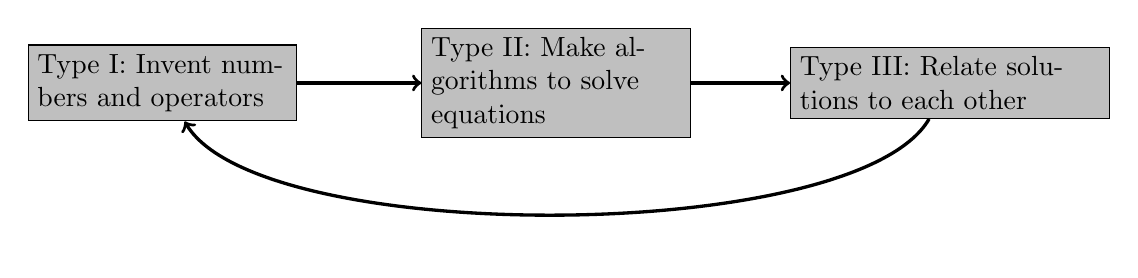
\begin{tikzpicture}
        \node[text width=1.25in, draw,fill=black!25] (a) at (0,0) {Type I: Invent numbers and operators};
        \node[text width=1.25in, draw,fill=black!25] (b) at (5,0) {Type II: Make algorithms to solve equations};
        \node[text width=1.5in, draw,fill=black!25] (c) at (10,0) {Type III: Relate solutions to each other};
        % \draw[very thick,->] (-4,0) -- (a);
        \draw[very thick,->] (a) -- (b);
        \draw[very thick,->] (b) -- (c);
        \draw[very thick,->] (c) edge[looseness=0.5,out=-120,in=-60] (a);
    \end{tikzpicture}
\end{center}
    
% \begin{enumerate}
%     \item What numbers lead to solutions existing? Do we need to invent $\sqrt{2}$
%     $i$, and possibly others?
%     \item If solutions exists, what algorithms find them? Complete the square, 
%         use a stock quadratic formula? Gaussian eliminate?
%     \item When multiple solutions, relate them to one another to simplify the answer.  
%     E.g.\ $\pm \sqrt{2}$, shift answers to a null space, use a basis.  Go 
%     back to 1 with these relations.
% \end{enumerate}

\section{$\mathbb{N}$: the first Type I algebra}
Childhood is mostly type I algebra.  Children learn to count and give these counts 
the usual names
\begin{center}
    % $0\defeq$ \underline{\hspace{5mm}}, 
    $1\defeq$ \StrokeOne,
    $2\defeq$ \StrokeTwo,
    $3\defeq$ \StrokeThree,
    $4\defeq$ \StrokeFour,
    $5\defeq$ \StrokeFive,...
\end{center}
Nothing gets the name $0$ (one theory is that the symbol reflects 
a dent in the sand left by removing the last pebble from a count.)
Mathematicians and programmers see these \emph{natural numbers}
as produced by two rules, start with nothing, $0$, or take a successor 
$S(k)$ to natural number $k$ already created.  In notation we separate the 
cases by $|$ (read as ``or'') and define $\mathbb{N}$ by this pattern
\begin{gather}
    \tag{Mathematics}
    \mathbb{N} = 0 | S(k)
\end{gather}
We say that $0$, $1\defeq S(0)$, $2\defeq S(S(0))$ and so on, are natural numbers.
It is important to see this as creating data rather than explaining data we 
already have.   To emphasize this 
point consider how this translates into programs, they wont be packages 
of known data, they will be ways to generate data.  Here and throughout 
we use coding displays in two of the three popular paradigms.

\begin{remark}
    In programming, logic is recorded by matching 
    a pattern of words and symbols called an \emph{idiom}.
    Often an idiom attempts to mimic a natural language
    (commonly English) or a mix of natural language and 
    mathematical notation.  A \emph{Programming Language (PL)}
    is a collection of idioms capable of expressing a 
    system of logic.  There are three major
    systems of logic, two based on functions, one based on 
    relations.  There are likewise three major PL families.
    \begin{description}
        \item[Procedural] PLs that express a 
        Lovelace-Turing-Curry \emph{Combinatorial Logic}, a logic 
        based on functions as sequences of primitive steps
        (combinators/assembly).  E.g. Fortan (1957-), C (1972-), 
        Python (1991-), Java (1995-).
    
        \item[Functional] PLs that express a 
        G\"odel-Church \emph{$\lambda$-calculus/recursive functions}, a logic 
        based on functions as substitution rules.
        E.g.\ Lisp (1960-), ML (1973-), Haskell (1990-). 
        
        \item[Relational] PLs that express a 
        Tarski-Codd \emph{Relational Logic}, a logic 
        based on relations rather than functions.
        E.g.\ SQL (1974-), Excel (1987-).
        
    \end{description}
    Most languages from 2000 and beyond use a mix of styles.
    We will concentrate on the first two families.    

    As a general guide, procedural PLs have preferred the 
    $\sin(x)$ style of functions where as functional PLs have 
    largely embraced the $\sin x$ convention.
\end{remark}

While dialects of languages differ, below are two pseudo-code samples 
repeating the definition $\mathbb{N}\defeq 0|S(k)$
in two of the dominant forms of programming.
\begin{center}
\begin{minipage}{0.9\textwidth}
    % $\mathbb{N} \defeq 0 \mid S(k)$\hfill (Mathematics)\\
\begin{minipage}{3in}
\begin{lstlisting}[language=Hidris]
data Nat = Z | S k
\end{lstlisting}
\end{minipage}\hfill (Functional Program)\\
            % \fcode{Nat = 0 | S k}\hfill (Functional Program)\\
\begin{minipage}{3in}
\begin{lstlisting}[language=Sava]
class Nat 
  case Zero ext Nat
  case Next(k:Nat) ext Nat
sealed
\end{lstlisting}
\end{minipage}\hfill (Procedural Program)\\
\end{minipage}
\end{center}


Writing $n\in \mathbb{N}$, $n:\mathbb{N}$,
\lstinline{0:Nat}, and
\lstinline{uint n} (represented an ``unsigned integer'')
are all ways that we communicate that we have some data 
$n$ that was created as a natural number.
This means when it comes time to use $n$ we can assume
one of two things $n=0$ or $n=S(k)$.  

\begin{example}
A function to decide if a natural number is positive.
    \begin{gather*}
        p(n) = \begin{cases}
            \top & n=0\\
            \bot & n=S(k)
        \end{cases}
    \end{gather*}
Here are some equivalents as programs.
\begin{center}
\begin{minipage}{2.5in}
\begin{lstlisting}[language=Hidris]
isPositive n = 
   match n with
         Z => true
     (S k) => false            
\end{lstlisting}
\end{minipage}
\hfill
\begin{minipage}{2in}
\begin{lstlisting}[language=Sava]
def isPos(n) = 
  match n with
    Zero    => true
    Next(k) => false            
\end{lstlisting}
\end{minipage}
\end{center}

                
\end{example}
For example, mathematicians might write
\begin{align*}
    p(n) & = \begin{cases}
        \top & n=0\\
        \bot & n=S(k)
    \end{cases}
    &
    e(n) & = \begin{cases}
        \top & n=0\\
        \bot & n=S(0)\\
        e(k) & n=S(S(k))
    \end{cases}
\end{align*}
The first function return $\top$ (which we read ``true'') if, and only if,
$n=0$; otherwise it returns $\bot$ (which reads as ``false'').  So $p$ is a test
of positivity.  Meanwhile $e$ uses an extra case so that $e(0)$ is true, $e(1)$
is false and $e(2+k)=e(k)$, where $2+k$ is short hand for $S(S(k))$.
Extrapolating the pattern, we end with true if, and only if, $n$ is even.
We could render these as code in roughly the same way but with idioms 
of a particular programming language.
\begin{center}
\begin{minipage}{0.45\textwidth}
\begin{lstlisting}[language=Hidris]
isPositive : Nat -> Boolean
isPositive 0 = true
isPositive (S k) = false
\end{lstlisting}
\end{minipage}
\begin{minipage}{0.45\textwidth}
\begin{lstlisting}[language=Hidris]
isEven: Nat->Boolean 
isEven n = match n with 
            0 => true 
            S 0 => false 
            S (S k) => isEven k
\end{lstlisting}
\end{minipage}
\end{center}
This creation of numbers inspires many others.
Imagine a string of characters in an alphabet \lstinline{Char:=['a','b',...,'z']}.
We start with either nothing (an empty string) or we add a character 
to a string we already have.  There is a little more going on here, we 
could add a character before or after the string we have.
\begin{lstlisting}[language=Hidris]
data String = Empty 
            | Prepend( head:Char, tail:String) 
            | Append( head:String, tail:Char)
\end{lstlisting}
Writing \lstinline{head:Char} or \lstinline{tail:String} 
indicates that head must come from the alphabet we chose 
and tail must be some already produced string, possibly empty.
Some readers might relate to a different dialect of 
programming such as the following
\begin{lstlisting}[language=Sava]
class String
  case Empty extends String
  case Prepend( head:Char, tail:String) extends String
sealed // No further cases
\end{lstlisting}
The head here caries around what we put in the list and the tail 
is what comes next in the list.  Observe the similarities:
\begin{align}
     2 & \defeq S(S(0)) \tag{$\mathbb{N}$}\\
 \text{\lstinline{"me"}} & \defeq \text{\lstinline{Prepend('m',Prepend('e',Empty))}}
\tag{String}
\end{align}
The left-hand sides are merely notation for what the data really is on the right.
Both the successor and the \lstinline{Prepend} are operators that generate 
new values.  So part of algebra is to generate new data; so, it is no wonder 
that it closely connections to computation.

\subsection*{Exercise}
\begin{enumerate}
    \item Mimic the String data type to make a list of integers (that is 
    switch from the alphabet to integers).

    \index{generics}
    \item Mimic the String data type to make a list of fixed by 
    unknown data of type $A$, call it \lstinline{List[A]}.\footnote{
    Alternatives include \lstinline{List a} and \lstinline{List<A>}. 
    Search for \emph{generics} in your programming language to learn more.
    }

\end{enumerate}
\index{nil}\index{cons}\index{list}
Historically \lstinline{Empty} for lists is called \lstinline{Nil} 
and \lstinline{Prepend} is called \lstinline{Cons}.


Children also learn to add, whatever that means conceptually, it obeys 
another simple pattern.
\begin{align*}
    m+n & \defeq\left\{ 
    \begin{array}{ll}
        n & m = 0\\
        S(n+k) & m=S(k)
    \end{array}
    \right.
\end{align*}
So does $2+4=6$?  We can test this out.
\begin{align*}
    \text{\StrokeTwo}+\text{\StrokeFour} & = \text{\StrokeOne}~ \big(\text{\StrokeOne} +\text{\StrokeFour}\big)\\
    & = \text{\StrokeOne}~ \big( \text{\StrokeOne}~\big(\underline{\hspace{5mm}}+\StrokeFour\big)\big)\\
    & = \text{\StrokeOne}~ \big( \text{\StrokeOne}~\StrokeFour\big)\\
    & = \text{\StrokeOne}~ \text{\StrokeFive}.
\end{align*}


A natural number is either $0$, or a successor 
$S(k)$ to 
another natural number $k$.  Often this is expressed as a 
definition where $\mid$ stands for separating cases, 
for example:
\begin{align*}
    \mathbb{N} \defeq 0 \mid S(k)
\end{align*}
So $0$ is ``zero'', and $1$ is just a symbol representing $S(0)$, 
$2\defeq S(S(0))$ and so on.  Replace $S$'s with tally marks (not to be 
confused with `$|$' used as an ``or'' above)
we recover childhood counting:
\begin{center}
    $0\defeq$ \underline{\hspace{5mm}}, 
    $1\defeq$ \StrokeOne,
    $2\defeq$ \StrokeTwo,
    $3\defeq$ \StrokeThree,
    $4\defeq$ \StrokeFour,
    $5\defeq$ \StrokeFive,...
\end{center}
The point is, the successors are not so much a function 
moving around the numbers we have, it actually is a producer 
of numbers. 
